\documentclass[tikz,border=8pt]{standalone}
\usepackage{amsmath,amssymb}
\usetikzlibrary{arrows.meta,calc,decorations.pathreplacing,patterns,shapes.geometric,positioning,shadings,plotmarks}

\begin{document}
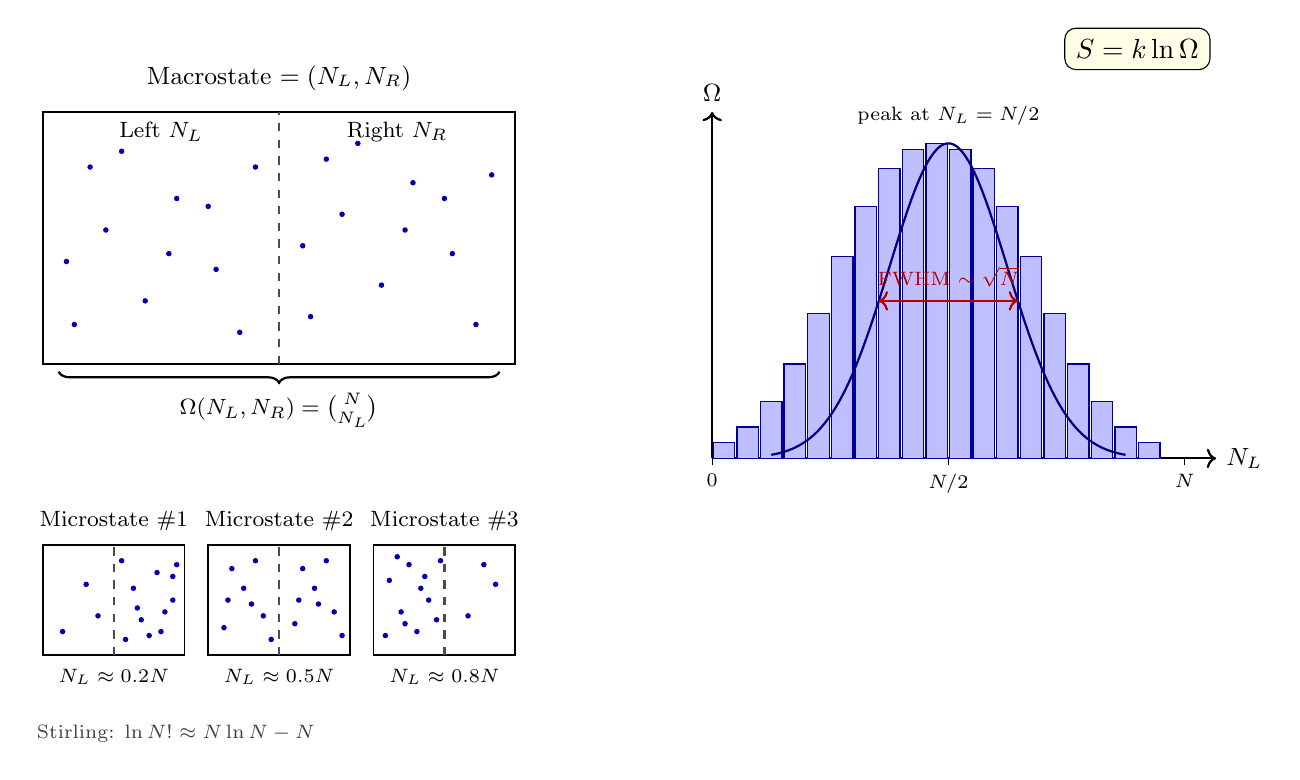
\begin{tikzpicture}[
  font=\small,
  particle/.style={circle, fill=blue!70!black, inner sep=0pt, minimum size=2pt},
  boxline/.style={thick, draw=black, line width=0.8pt},
  divider/.style={dashed, thick, draw=black!70},
  microbox/.style={draw=black, line width=0.6pt},
  histbar/.style={draw=blue!60!black, fill=blue!25, line width=0.5pt},
]

% =====================================================
% LEFT: Big macrostate box with random particles
% =====================================================
\def\bigW{6}
\def\bigH{3.2}

% Title above big box
\node[anchor=south] at (\bigW/2, \bigH+0.15) {Macrostate $= (N_L, N_R)$};

% Big box outline
\draw[boxline] (0,0) rectangle (\bigW,\bigH);
% Center vertical dashed divider
\draw[divider] (\bigW/2,0) -- (\bigW/2,\bigH);

% Labels for halves
\node at (\bigW/4, \bigH-0.25) {\footnotesize Left $N_L$};
\node at (3*\bigW/4, \bigH-0.25) {\footnotesize Right $N_R$};

% Random particles - "uniform" macrostate (left ~ right)
% Left side (12 particles)
\foreach \x/\y in {
  0.4/0.5, 0.8/1.7, 1.3/0.8, 1.7/2.1, 0.6/2.5, 2.2/1.2,
  2.5/0.4, 1.0/2.7, 2.7/2.5, 0.3/1.3, 2.1/2.0, 1.6/1.4
}{ \node[particle] at (\x,\y) {}; }
% Right side (12 particles)
\foreach \x/\y in {
  3.4/0.6, 3.8/1.9, 4.3/1.0, 4.7/2.3, 3.6/2.6, 5.2/1.4,
  5.5/0.5, 4.0/2.8, 5.7/2.4, 3.3/1.5, 5.1/2.1, 4.6/1.7
}{ \node[particle] at (\x,\y) {}; }

% =====================================================
% Three microstate examples below
% =====================================================
\def\smY{-2.6}     % center y
\def\smYbot{-3.7}  % bottom of small boxes
\def\smYtop{-1.5}  % top of small boxes
\def\smW{1.8}
\def\smH{1.4}

% Microstate #1: N_L approx 0.2 N (mostly right)
\def\xa{0.0}
\draw[microbox] (\xa,\smYbot) rectangle (\xa+\smW,\smYbot+\smH);
\draw[divider]  (\xa+\smW/2,\smYbot) -- (\xa+\smW/2,\smYbot+\smH);
% Few on left (3), many on right (12)
\foreach \dx/\dy in {0.25/0.3, 0.55/0.9, 0.7/0.5}{
  \node[particle] at (\xa+\dx,\smYbot+\dy) {};
}
\foreach \dx/\dy in {
  1.05/0.2, 1.25/0.45, 1.5/0.3, 1.65/0.7, 1.15/0.85, 1.45/1.05,
  1.7/1.15, 1.0/1.2, 1.55/0.55, 1.35/0.25, 1.65/1.0, 1.2/0.6
}{ \node[particle] at (\xa+\dx,\smYbot+\dy) {}; }
\node[anchor=south, font=\footnotesize] at (\xa+\smW/2, \smYbot+\smH+0.05)
  {Microstate \#1};
\node[anchor=north, font=\scriptsize] at (\xa+\smW/2, \smYbot-0.05)
  {$N_L \approx 0.2N$};

% Microstate #2: N_L approx 0.5 N (uniform)
\def\xb{2.1}
\draw[microbox] (\xb,\smYbot) rectangle (\xb+\smW,\smYbot+\smH);
\draw[divider]  (\xb+\smW/2,\smYbot) -- (\xb+\smW/2,\smYbot+\smH);
\foreach \dx/\dy in {
  0.2/0.35, 0.45/0.85, 0.7/0.5, 0.3/1.1, 0.6/1.2, 0.8/0.2,
  0.55/0.65, 0.25/0.7
}{ \node[particle] at (\xb+\dx,\smYbot+\dy) {}; }
\foreach \dx/\dy in {
  1.1/0.4, 1.35/0.85, 1.6/0.55, 1.2/1.1, 1.5/1.2, 1.7/0.25,
  1.4/0.65, 1.15/0.7
}{ \node[particle] at (\xb+\dx,\smYbot+\dy) {}; }
\node[anchor=south, font=\footnotesize] at (\xb+\smW/2, \smYbot+\smH+0.05)
  {Microstate \#2};
\node[anchor=north, font=\scriptsize] at (\xb+\smW/2, \smYbot-0.05)
  {$N_L \approx 0.5N$};

% Microstate #3: N_L approx 0.8 N (mostly left)
\def\xc{4.2}
\draw[microbox] (\xc,\smYbot) rectangle (\xc+\smW,\smYbot+\smH);
\draw[divider]  (\xc+\smW/2,\smYbot) -- (\xc+\smW/2,\smYbot+\smH);
\foreach \dx/\dy in {
  0.15/0.25, 0.35/0.55, 0.55/0.3, 0.7/0.7, 0.2/0.95, 0.45/1.15,
  0.65/1.0, 0.8/0.45, 0.3/1.25, 0.6/0.85, 0.85/1.2, 0.4/0.4
}{ \node[particle] at (\xc+\dx,\smYbot+\dy) {}; }
\foreach \dx/\dy in {1.2/0.5, 1.55/0.9, 1.4/1.15}{
  \node[particle] at (\xc+\dx,\smYbot+\dy) {};
}
\node[anchor=south, font=\footnotesize] at (\xc+\smW/2, \smYbot+\smH+0.05)
  {Microstate \#3};
\node[anchor=north, font=\scriptsize] at (\xc+\smW/2, \smYbot-0.05)
  {$N_L \approx 0.8N$};

% Bracket connecting big box to microstates
\draw[decorate, decoration={brace, amplitude=4pt, mirror}, thick]
  (0.2,-0.1) -- (\bigW-0.2,-0.1)
  node[midway, below=4pt, font=\footnotesize]
  {$\Omega(N_L,N_R) = \binom{N}{N_L}$};

% =====================================================
% RIGHT: Histogram of Omega(N_L)
% =====================================================
\def\hxo{8.5}     % histogram x-origin
\def\hyo{-1.2}    % histogram y-origin
\def\hW{6.0}      % histogram width
\def\hH{4.0}      % histogram height

% Axes
\draw[->, thick] (\hxo,\hyo) -- (\hxo+\hW+0.4,\hyo) node[right] {$N_L$};
\draw[->, thick] (\hxo,\hyo) -- (\hxo,\hyo+\hH+0.4) node[above] {$\Omega$};

% Tick marks at 0, N/2, N
\draw (\hxo,\hyo) -- (\hxo,\hyo-0.08) node[below, font=\scriptsize] {$0$};
\draw (\hxo+\hW/2,\hyo) -- (\hxo+\hW/2,\hyo-0.08)
  node[below, font=\scriptsize] {$N/2$};
\draw (\hxo+\hW,\hyo) -- (\hxo+\hW,\hyo-0.08)
  node[below, font=\scriptsize] {$N$};

% Histogram bars: discretized Gaussian centered at N/2 with sigma ~ sqrt(N)/2
% We model 21 bars, peak at center = bar 10
% Heights based on exp(-((i-10)/3)^2) scaled to hH
\foreach \i/\h in {
  0/0.05,  1/0.10,  2/0.18,  3/0.30,  4/0.46,
  5/0.64,  6/0.80,  7/0.92,  8/0.98,  9/1.00,
 10/0.98, 11/0.92, 12/0.80, 13/0.64, 14/0.46,
 15/0.30, 16/0.18, 17/0.10, 18/0.05
}{
  \pgfmathsetmacro{\bx}{\hxo + (\i+0.5)*\hW/20.0}
  \pgfmathsetmacro{\bw}{\hW/22.0}
  \pgfmathsetmacro{\bh}{\h*\hH}
  \draw[histbar] (\bx-\bw/2,\hyo) rectangle (\bx+\bw/2,\hyo+\bh);
}

% Smooth Gaussian envelope overlay
\draw[thick, blue!50!black, smooth, samples=80, domain=-3.0:3.0]
  plot ({\hxo + (\hW/2) + \x*(\hW/8)}, {\hyo + \hH*exp(-\x*\x/2)});

% FWHM bracket near top of bell, indicating ~ sqrt(N)
\pgfmathsetmacro{\hwhmL}{\hxo + \hW/2 - 1.18*\hW/8}
\pgfmathsetmacro{\hwhmR}{\hxo + \hW/2 + 1.18*\hW/8}
\pgfmathsetmacro{\hwhmY}{\hyo + \hH*0.5}
\draw[<->, thick, red!70!black] (\hwhmL,\hwhmY) -- (\hwhmR,\hwhmY);
\node[font=\scriptsize, red!70!black, above]
  at ({(\hwhmL+\hwhmR)/2}, \hwhmY+0.05) {FWHM $\sim \sqrt{N}$};

% Peak label
\node[font=\scriptsize] at (\hxo+\hW/2, \hyo+\hH+0.35) {peak at $N_L=N/2$};

% Boltzmann formula box (top right)
\node[draw=black, fill=yellow!10, rounded corners, inner sep=4pt,
      font=\normalsize]
  at (\hxo+\hW-0.6, \hyo+\hH+1.2) {$S = k\ln\Omega$};

% Stirling approximation note (bottom-left of figure)
\node[anchor=west, font=\scriptsize, gray!50!black]
  at (-0.2, -4.7)
  {Stirling: $\ln N! \approx N\ln N - N$};

\end{tikzpicture}
\end{document}
